\documentclass[12pt]{scrreprt}

%\documentclass[a4paper, 12pt, oneside]{scrbook}

%Eingaben

\usepackage[latin1, utf8]{inputenc}

\usepackage[T1]{fontenc}

\usepackage[ngermanb, english]{babel}

\usepackage{amsmath}
\usepackage{amsthm}
\usepackage{ulem}
%Layout

\usepackage{lmodern}

\usepackage{hyperref}

\usepackage[all]{hypcap} %Bei Verlinkungen auf Bilder die obere Grenze des Bildes verkinken.

%Für die Erzeugung von Graphiken

\usepackage{tikz}

%\usepackage{graphicx}

%Quellcode

\usepackage{listings}
\usepackage{graphicx}
\usepackage{color}

\lstdefinestyle{Shell}{delim=[il][\bfseries]{BB}}

\lstset{flexiblecolumns = true}

%

\usepackage[verbose]{placeins}

\usepackage{float} % for option H

% code highlighting

\usepackage{listings}
\usepackage{color}
 
\definecolor{codegreen}{rgb}{0,0.6,0}
\definecolor{codegray}{rgb}{0.5,0.5,0.5}
\definecolor{codepurple}{rgb}{0.58,0,0.82}
\definecolor{backcolour}{rgb}{0.95,0.95,0.92}
 
\lstdefinestyle{mystyle}{
    backgroundcolor=\color{backcolour},   
    commentstyle=\color{codegreen},
    keywordstyle=\color{magenta},
    numberstyle=\tiny\color{codegray},
    stringstyle=\color{codepurple},
    basicstyle=\footnotesize,
    breakatwhitespace=false,         
    breaklines=true,                 
    captionpos=b,                    
    keepspaces=true,                 
    numbers=left,                    
    numbersep=5pt,                  
    showspaces=false,                
    showstringspaces=false,
    showtabs=false,                  
    tabsize=2
}
 
\lstset{style=mystyle}


%\usepackage{siunitx}%schreibt einheiten richtig mit gutem abstand und richtige schriftzeichen
%\[v=\SI{2.3}{\metre\per\second}]
%\sisetup{% DE macht komma;
%  locale = UK%,
  %group-separator = {.} %,
  %per-mode = symbol
%}klappt irgendwie nicht so wie es soll


    \usepackage{xcolor} % Allow colors to be defined
    \usepackage{upquote} % Upright quotes for verbatim code
    \usepackage{fancyvrb} % verbatim replacement that allows latex
    \newcommand{\VerbatimStringTok}[1]{\textcolor[rgb]{0.25,0.44,0.63}{{#1}}}




\usepackage[scaled]{beramono}

\lstset{
  language=Python
}
\usepackage{enumitem}


    % Exact colors from NB
    \definecolor{incolor}{rgb}{0.0, 0.0, 0.5}
    \definecolor{outcolor}{rgb}{0.545, 0.0, 0.0}

    \DefineVerbatimEnvironment{Highlighting}{Verbatim}{commandchars=\\\{\}}


\begin{document}
%\titlehead{}
\subject{Data Science}
\title{Documentation}
\subtitle{Nearest Neighbors - Advanced (LSH)}
\author{}
\date{\large{\today}}
\publishers{Eicker Niklas, Halastra Szymon}
%\extratitle{\centering Schmutztitel}
%\uppertitleback{Obiger Titelrückentitel}
%\lowertitleback{Unterer Rückseitentitel}
%\dedication{Rückseite der Titelseite}
\maketitle
\tableofcontents



\chapter{Introduction} 
\label{chpt:intro}

Using GraphLab Create we will load and analyze data on Wikipedia articles about persons. In this advanced project we will use Locality Sensitive Hashing (LSH) to achieve fast and efficient approximate nearest neighbor searches.

\section{The data set}
\label{sec:data}

Each element of the original data set consists of a link to a Wikipedia article, the name of the person it is about and the text of the article (in lowercase and without punctuation). There are 59071 entries in total. An excerpt of the data "as is" can be seen in figure \ref{fig:dataset_raw}.\\


\begin{figure}[H]
  \begin{center}
    \caption{Excerpt of the data set.}
    \label{fig:dataset_raw}
    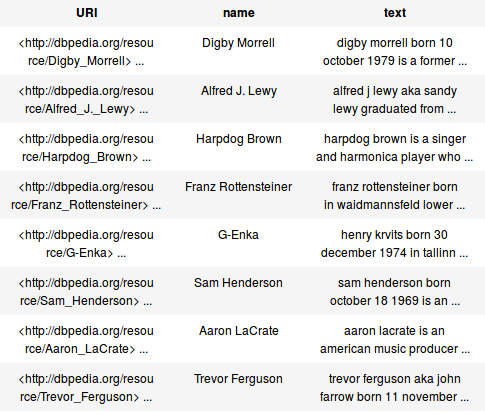
\includegraphics[width=0.8\textwidth, angle=0]{raw_data.jpg}
  \end{center}
\end{figure}

\chapter{Data preparation}
\label{chpt:tasks}

As preparation we add a new column to the data set containing the TF-IDF values as well as a row count acting as unique article ID.\\

The GraphLab Create method 'text\_analytics.tf\_idf' calculates TF-IDF values for all our articles. Adding the ID id done via an in-build method of the SFrame 'add\_row\_number'. A short preview of the modified data set can bee seen in figure \ref{fig:dataset}.\\

\begin{figure}[H]
  \begin{center}
    \caption{Preview of the data set with an additional column for TF-IDF and unique IDs.}
    \label{fig:dataset}
    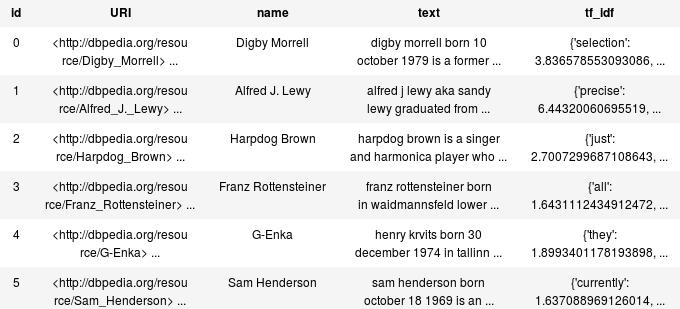
\includegraphics[width=0.95\textwidth, angle=0]{db_wiki_word_counts_and_id.jpg}
  \end{center}
\end{figure}

For the rest of the assignment we will use sparse matrices instead of the SFrame. A sparse matrix is a matrix with only a few non zero elements. SciPy supports this format and allows us to easily handle our TF-IDF values in matrix form. First we have to convert the original dictionary structure to the new SciPy sparse matrix format.\\

We transform the TF-IDF dictionaries in one 59071 x 547979 sparse matrix, where each row is a document and each column a word. Now every document has a TF-IDF value for every word in any document. If the word does not appear in the document, which is the case for most words, the value is zero.\\


\chapter{Locality Sensitive Hashing}

LSH is a hashing method that aims to maximize the probability of a "collision" for similar items. Via randomly generated vectors we will assign each document to a specific bin. The total number of bins should be chosen in a way, that the bin of a queried document and it's surrounding bins include the "real" nearest neighbors. Due to the smaller amount of the documents in surrounding bins (compared to the complete sample), it will be possible to calculate the closest neighbors faster then by brute force.\\


\section{Sorting data into bins}
For the beginning we have to decide on a number of random vectors. This number will define the number of bins. With each vector we will generate one bit for every document by multiplying it with the document's TF-IDF vector and checking the sign of the solution. Each unique combination of bits represents one data bin.\\

We create 16 Gaussian random vectors, which will yield $2^{16}$ (65536) bins to sort our data into. In this case the number of bins is comparable to the number of documents in the data set.\\

Each scalar product with a document and all random vectors gives us an array of Boolean with the length of 16 (= number of vectors). We can transform this array into an ID for the corresponding bin, by taking it as a 16-bit binary number and calculating it's single integer value. At this point we have sorted all our documents into bins and can start to compare single documents to other documents inside the same bin and surrounding bins.\\

\newpage
\section{First evaluation of a LSH model}
With every document in it's corresponding bin, we can take a look at the actual "closeness" of documents in the same and surrounding bins. To measure the closeness we will be using the cosine distance, which was closer investigated in the primer task.\\

As an example we will be using the Wikipedia page of Barack Obama. In Obama's bin there are five other pages. Table \ref{tab:compare_top_words} lists the names and cosine distances of these documents to Barack Obama's article. Most of them are far away from Barack Obama with cosine distances above $0.9$, but the closest is Joe Biden with a distance of $0.7$. It is obvious, that LSH is just an approximation and one has to consider documents from surrounding bins to find the real nearest neighbors.

\begin{table}[H]
  \caption{Comparison of the documents that share the same bin as Back Obama's article.}
  \label{tab:compare_top_words}
  \begin{center}
    \begin{tabular}{| c | c | c |}
      \hline
      \textbf{Rank} & \textbf{Name} & \textbf{Distance to Obama}\\
      \hline
      \hline
      1 & Joe Biden & 0.703139 \\ \hline
      2 & Mark Boulware & 0.950867 \\ \hline
      3 & John Wells (politician) & 0.975966 \\ \hline
      4 & Francis Longstaff & 0.978256 \\ \hline
      5 & Madurai T. Srinivasan & 0.993092 \\ \hline
    \end{tabular}	
  \end{center}
\end{table}

\chapter{Querying the LSH model}
\section{Structure of a query}
In the previous chapter we found that a query of our model will have to take surrounding bins into account. One can define a range for such a query as the number of different bits in the bins bit representations. Such a query with the range 3 will look like this:\\
\begin{center}
\begin{enumerate}
\item[1.] Let L be the bit representation of the bin that contains the query documents.
\item[2.] Consider all documents in bin L.
\item[3.] Consider documents in the bins whose bit representation differs from L by 1 bit.
\item[4.] Consider documents in the bins whose bit representation differs from L by 2 bits.
\item[5.] Consider documents in the bins whose bit representation differs from L by 3 bits.
\end{enumerate}
\end{center}

\section{Query implementation}
For an easy implementation of the query we use "itertools.combinations". This method takes the number of our vectors (number of bits in a bin ID) and the query range. It returns a collection of lists, which show all possible bit flips that lead to surrounding bins with the given range as maximum number of flips. Our query method takes these lists of bit flips, applies each one of them and saves all documents found in any of the reached bins in a set. This set then includes all possible candidates for being nearest neighbors and can be further examined.\\

The first part of the query gives us a set of candidates. From this set we compute the true cosine distances of the candidates to the queried document and then take a look at the top 10. The names and distances of the results for a query radius of 3 can be found in table \ref{tab:top_10_range_3} and are a lot better then the results from just looking at the other documents in the same bin.\\

\begin{table}[H]
  \caption{Top ten nearest neighbors for Barack Obama. This data is obtained with 16 random vectors and a search range of 3.}
  \label{tab:top_10_range_3}
  \begin{center}
    \begin{tabular}{| c | c | c |}
      \hline
      \textbf{Rank} & \textbf{Name} & \textbf{Distance to Obama}\\
      \hline
      \hline
      1 & Barack Obama & 0 \\ \hline
      2 & Joe Biden & 0.703 \\ \hline
      3 & Nathan Cullen & 0.857 \\ \hline
      4 & Barry Sullivan (lawyer) & 0.875 \\ \hline
      5 & Neil MacBride & 0.89 \\ \hline
      6 & Vikramaditya Khanna & 0.898 \\ \hline
      7 & Herman Cain & 0.899 \\ \hline
      8 & Raymond F. Clevenger & 0.901 \\ \hline
      9 & Michael J. Malbin & 0.903 \\ \hline
      10 & Lowell Barron & 0.909 \\ \hline
    \end{tabular}	
  \end{center}
\end{table}

\chapter{Tuning of the LSH model}
There are two main aspects of our model that we would like to tune.\\
\begin{center}
\begin{enumerate}
\item[1.] \textbf{Speed}\\
The faster the query the better. This is why we use an approximate technique like LSH in the first place.
\item[2.] \textbf{Accuracy}\\
Speed is nice, but the search results should still be close to the exact results by brute force.
\end{enumerate}
\end{center}

\section{The range parameter}
\label{sec:range}
The range parameter affects our queries by defining the number of bins searched. This also affects the number of documents for the exact distance calculation. Thus both speed and accuracy can be tuned with this parameter.\\

To take a closer look at the affect of the range parameter we will query Obama once more, but this time with ranges from 0 to 16 while recording the query time and results. Figure \ref{fig:docs_93} shows how the number of considered documents raises with the search radius. On the other hand, more documents also mean longer query times, as can be seen in figure \ref{fig:time_93}. Figure \ref{fig:accuracy_93} finally shows the raising accuracy of our search, while we are approaching the brute force results.\\

This evaluation is only for an "Obama query". We repeated it for 10 randomly chosen documents and recorded the time per query and how many of the top 10 where in the top 25 of brute force. The later precision measurement can be seen in figure \ref{fig:dataset}. The results look similar to the single query results with Obama. With a range of 7 we get precise top 10 documents and still have a time advantage over brute force (<50\%).\\

\begin{figure}[H]
  \begin{center}
    \caption{Number of documents searched for different search radii.}
    \label{fig:docs_93}
    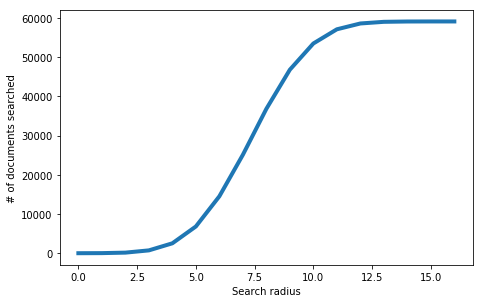
\includegraphics[width=0.8\textwidth, angle=0]{output/output_93_0.png}
  \end{center}
\end{figure}
\begin{figure}[H]
  \begin{center}
    \caption{Time elapsed for one query with changing search radius.}
    \label{fig:time_93}
    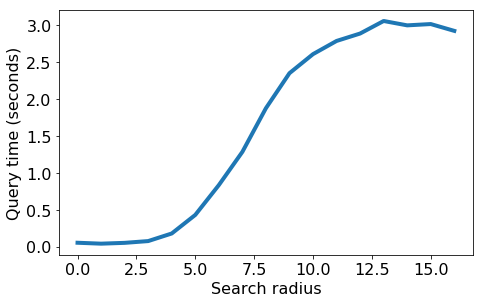
\includegraphics[width=0.8\textwidth, angle=0]{output/output_93_1.png}
  \end{center}
\end{figure}
\begin{figure}[H]
  \begin{center}
    \caption{Distances of the top 10 documents to the queried article.}
    \label{fig:accuracy_93}
    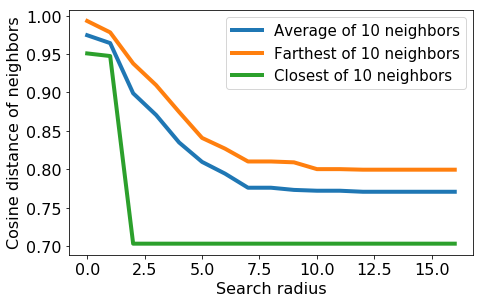
\includegraphics[width=0.8\textwidth, angle=0]{output/output_93_2.png}
  \end{center}
\end{figure}

\begin{figure}[H]
  \begin{center}
    \caption{Precision of the top 10 query compared to the top 25 of brute force.}
    \label{fig:accuracy_93}
    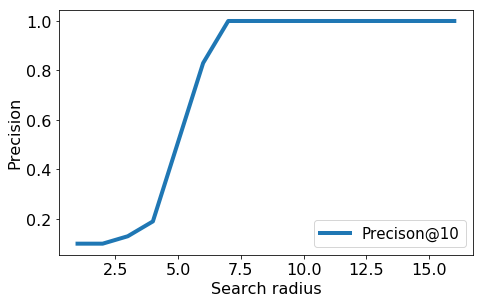
\includegraphics[width=0.8\textwidth, angle=0]{output/output_103_1.png}
  \end{center}
\end{figure}

\section{The number of random vectors}
\label{sec:vectors}
To asses the effects of a changing number of random vectors, we pick 10 random documents and query them with a fixed range of 3 and vary the number of random vectors between 5 and 19.\\

As with the range parameter there is a trade off between precision and query time. With less vectors, the documents are split into less bins and a search with fixed range will look through more documents. This raises the precision, but also makes the queries slower. Figure \ref{fig:precision} shows the falling precision with more random vectors, while figure \ref{fig:speed} visualizes the faster queries. Keep in mind that this all happens at range 3.\\

\begin{figure}[H]
  \begin{center}
    \caption{Precision of the top 10 being in the top 25 of brute force. (Range = 3)}
    \label{fig:precision}
    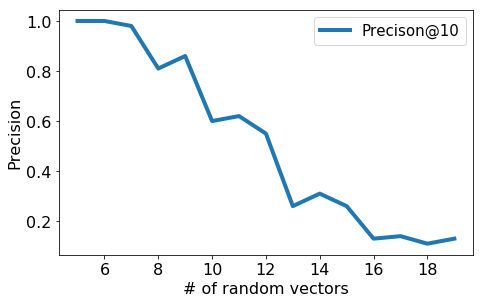
\includegraphics[width=0.8\textwidth, angle=0]{output/output_108_1.png}
  \end{center}
\end{figure}
\begin{figure}[H]
  \begin{center}
    \caption{Time elapsed during one query. (Range = 3)}
    \label{fig:speed}
    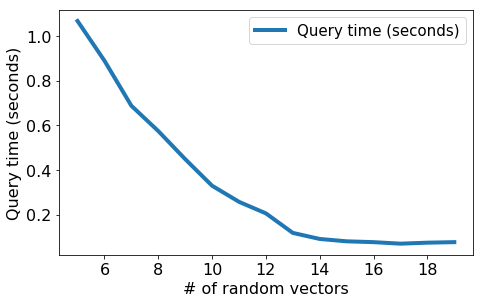
\includegraphics[width=0.8\textwidth, angle=0]{output/output_108_2.png}
  \end{center}
\end{figure}

\section{Balancing the parameters}
We found that a range of 3 in section \ref{sec:vectors} was a bit low, when looking at the analysis in section \ref{sec:range}. Out of interest we changed the range to 5 and repeated the analyses for 10 random documents with the number of random vectors between 5 and 19. Figure \ref{fig:pressision_2} shows, that we still get a precision of 1 for 11 random vectors at an astonishing 0.75s per query (\ref{fig:speed_2}).\\


\begin{figure}[H]
  \begin{center}
    \caption{Precision of the top 10 being in the top 25 of brute force. (Range = 5)}
    \label{fig:pressision_2}
    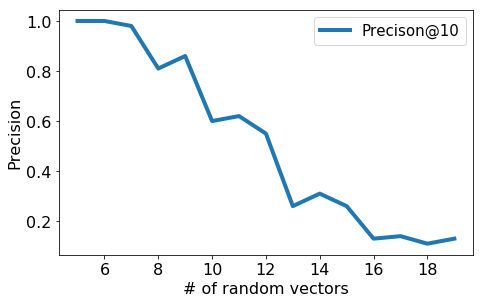
\includegraphics[width=0.8\textwidth, angle=0]{output/output_108_1.png}
  \end{center}
\end{figure}
\begin{figure}[H]
  \begin{center}
    \caption{Time elapsed during one query. (Range = 5)}
    \label{fig:speed_2}
    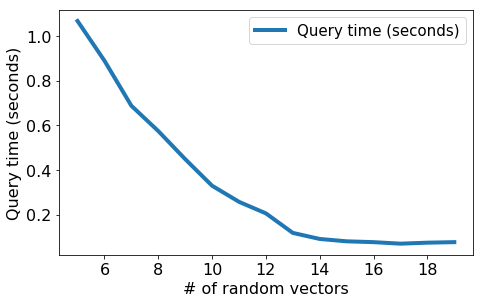
\includegraphics[width=0.8\textwidth, angle=0]{output/output_108_2.png}
  \end{center}
\end{figure} 



\end{document}